\documentclass[11pt,a4paper]{article}
\usepackage{moesiom} %estilo Moésio
%-----------------------------------------------------------
\usepackage{mathtools}
\usepackage{bookmark}
\usepackage{xargs} % Use more than one optional parameter in a new commands
\usepackage[pdftex,dvipsnames]{xcolor}  % Coloured text etc.
%\usepackage{xcolor}  % Coloured text etc.
\usepackage{polynom}
%-----------------------------------------------------------
\usepackage{pgfmath}
\usepackage{tkz-euclide}
\usepackage{tikz}
\usepackage{calculator}
%\usetikzlibrary{fit,arrows.meta,shadows,decorations.pathreplacing,calc}
%\tikzset{>=latex} % for LaTeX arrow head
\pgfplotsset{compat=1.13}
\usepackage{pgfplots}
%-----------------------------------------------------------
%
%
\usepackage[colorinlistoftodos,prependcaption,linecolor=red,backgroundcolor=blue!25,bordercolor=blue,textsize=tiny]{todonotes}
%\newcommandx{\unsure}[2][1=]{\todo[linecolor=red,backgroundcolor=red!25,bordercolor=red,#1]{#2}}
%-----------------------------------------------------------
\usepackage[url,doi,style=numeric,backend=biber]{biblatex}
\addbibresource{ref.bib}
%-----------------------------------------------------------
\newcommand{\nomer}{\bf Moésio M. de Sales\footnote{moesio@ifce.edu.br}}
\newcommand{\nome}{\bf Moésio M. de Sales}
\newcommand{\nomet}{\bf Moésio M. de Sales}
\newcommand{\titu}{Provas e Soluções}
\newcommand{\subtitu}{Concurso}
\newcommand{\disc}{Aulas}
\newcommand{\curso}{Formações}
\newcommand{\inst}{IFCE}
%-----------------------------------------------------------
\newcommand{\Z}{{\mathbb Z}}
\newcommand{\N}{{\mathbb N}}
\newcommand{\R}{{\mathbb R}}
\newcommand{\Mod}[1]{\ (\mathrm{mod}\ #1)}
%\renewcommand{\qed}{\hfill\blacksquare}
%-----------------------------------------------------------
\usepackage{tikz}
\usetikzlibrary{fit, shapes.geometric, arrows}
\newcommand{\DEF}[1]{\noindent
\colorbox{gray!10}{\begin{minipage}[t]{.89\textwidth}\centering
\begin{Def} #1 \end{Def} \end{minipage}}}
\newcommand{\PROP}[1]{\noindent
\colorbox{blue!10}{\begin{minipage}[t]{.89\textwidth}\centering
\begin{Prop} #1 \end{Prop} \end{minipage}}}
\newcommand{\teo}[2]{\noindent
\colorbox{red!10}{\begin{minipage}[t]{.89\textwidth}\centering
\begin{Teo}[#1] #2 \end{Teo} \end{minipage} }\\ }
\newcommand{\Obs}[1]{\noindent
\colorbox{gray!10}{\begin{minipage}[t]{.89\textwidth}\centering
\begin{obs} #1 \end{obs} \end{minipage}}}
\newcommand{\EXE}[1]{\noindent
\colorbox{gray!10}{\begin{minipage}[t]{.89\textwidth}\centering
\begin{exe} #1 \end{exe} \end{minipage}}}
\newcommand{\qst}[1]{\noindent
\colorbox{blue!10}{\begin{minipage}[t]{.89\textwidth}
		 #1  \end{minipage}}}
\newcommand{\SOL}[1]{\noindent
\colorbox{red!10}{\begin{minipage}[t]{.89\textwidth}
\begin{sol} #1 \end{sol} \end{minipage}}}
%
%-----------------------------------------------------------
%comando para compilar 
%pdflatex --enable-write18 -interaction=nonstopmode %.tex
%-----------------------------------------------------------
\begin{document}
{\Large
\begin{center} \titu\\ \disc\\  \nome\end{center}
}
%-----------------------------------------------------------
\hfill   %\today\\[2mm]
\hrule\ 
%-----------------------------------------------------------
%Prova de 2016 
%Questões 31, 32, 33, 35, 36, 37, 38, 39 ,40 
%42, 41, 43,( tenho dúvida se fiz certo)

%Prova de 2018 
%Questões 47, 33, 34 ( tenho dúvidas se fiz certo)
%-----------------------------------------------------------
\section{Prova 2016}
Veja~\cite{Ed1976teoria}

\qst{
{\bf Questão 31} O produto $x.y$ é igual a $338$. Adicionando~se $3$ 
unidades a cada um dos números ($x$ e $y$), o novo produto é $464$.
A soma $x+y$ vale:
\begin{multicols}{4}
\begin{enumerate}
		\item ( ) 28.
		\item ( ) 39.
		\item ( )171.
		\item ( ) 339.
\end{enumerate}
\end{multicols}

}
\SOL{
A soma $x+y$ vale:
\begin{eqnarray*}
		\begin{cases}
				x\cdot y = 338\\
				(x+3)(y+3) = 464
		\end{cases}\\
		\text{Na segunda equação}\\
		(x+3)(y+3) =xy+3x+3y+9 &= & 464\\
						xy+3(x+y)+9 &= & 464\\
						338+3(x+y)+9 &= & 464\\
						3(x+y)+347 &= & 464\\
						(x+y)&= & \frac{464-347}{3} = \frac{117}{3}  =  39
\end{eqnarray*}

}
%
\qst{
{\bf Questão 32} 
A expressão $0,000028$ pode ser representada através da potência:
\begin{multicols}{2}
\begin{enumerate}
		\item ( )$ 2,8 \times 10^{-5}$.
		\item ( )$ 2,8 \times 10^{-4}$.
\item ( )$ 2,8 \times 10^4$.
\item ( )$ 2,8 \times 10^5$.
\end{enumerate}
\end{multicols}

}
\SOL{
\begin{eqnarray*}
		0,000028 = \frac{2,8}{100000}=2,8 \times 10^{-5}
\end{eqnarray*}

}
%%
\qst{
{\bf Questão 33} 
João, José, Pedro e Tiago estãc em um restaurante e pedem uma pizza. Ao chegar o pedido, eles percebem
que a pizza não veio fatiada. Eles decidem entre si a seguinte divisão: João comerá $1/8$ da pizza, José comerá $9/40$
e Pedro comerá $17/80$ da pízza. Desta forma, sobrará para Tiago;
\begin{multicols}{2}
\begin{enumerate}
		\item ( )$ 14/40$ da pízza.
		\item ( )$ 17/32$ da pizza.
		\item ( )$ 7/16$ da pízza.
		\item ( )$ 1/2$ da pizza.
\end{enumerate}
\end{multicols}

}
\SOL{
\begin{eqnarray*}
		\frac{1}{8}+\frac{9}{40}+\frac{17}{80}&= & 
		\frac{10\times 1+2\times 9+17}{80}\\
		 &= & \frac{10+18+17}{80}\\
		 &= & \frac{45}{80}= \frac{9}{16}\\
		 \text{Sobrando} 
		 &= & 1-\frac{9}{16}= \frac{16-9}{16}= \frac{7}{16}
\end{eqnarray*}

}
%\queb
%%
\qst{
{\bf Questão 35} 
Uma mulher compra $5$ canetas e $3$ lápis pagando um valor total de $R\$ 14,50$. Um mês depois ela retorna à
mesma loja para comprar $8$ canetas e $5$ lápis e paga $R\$ 23,50$. Supondo que não houve variação nos preços,
assinale o valor de cada caneta e de cada lápis:
\begin{enumerate}
		\item ( ) A caneta custa $R\$ 1,50$ e o lápis $R\$ 2,00$.
		\item ( ) A caneta custa $R\$ 1,00$ e o lápis $R\$ 2,50$.
		\item ( ) A caneta custa $R\$ 2,50$ e o lápis $R\$ 1,00$.
		\item ( ) A caneta custa $R\$ 2,00$ e o lápis $R\$ 1,50$.
\end{enumerate}

}
%
\SOL{
\begin{eqnarray*}
		\text{Sejam x e y os valores por unidades das canetas e lápis, respectivamente}\\
		\begin{cases}
				5x+3y=14,50\\
				8x+5y=23,50
		\end{cases}\\
		\text{Resolvendo o sistema}
		\begin{cases}
				5x+3y=14,50 (\times -8)\\
				8x+5y=23,50 (\times 5)
		\end{cases}
		\Rightarrow
		\begin{cases}
				-40x-24y=-116\\
				40x+25y=117,5
		\end{cases}\\
		\text{Somando}\  
		y=117,5-116 =1,5\\
		\text{Substituindo}\ 
		5x+3y=14,50\ \Rightarrow 5x+3(1,5)=14,50 \Rightarrow x =\frac{14,5-4,5}{5}=2
\end{eqnarray*}

}
%%
\qst{
{\bf Questão 36} 
 Para comprar camisas e calções, um homem dispõe de uma certa quantia. Na loja $A$ o calção custa $R\$ 40,00$ e
a camisa custa $R\$ 60,00$. Já na loja $B$, o calção custa $R\$ 35,00$ e a camisa custa $R\$ 70,00$. Independentemente da
escolha da loja, o número de calções comprados não mudará. O mesmo vale para o número de camisas. Nestas
condições, para que o valor total da compra seja o mesmo em ambas as lojas:

\begin{enumerate}
		\item ( ) a quantidade de calções deve ser igual à quantidade de camisas.
		\item ( ) a quantidade de calções deve ser o dobro da quantidade de camisas.
		\item ( ) a quantidade de calções deve ser a metade da quantidade de camisas.
		\item ( ) a quantidade de calções deve ser um terço da quantidade de camisas.
\end{enumerate}

}
\SOL{
\begin{eqnarray*}
		\text{Sejam x e y as quantidades de calções e camisas, respectivamente}\\
		\begin{cases}
				40x+60y=\text{preço em A}\\
				35x+70y=\text{preço em B}
		\end{cases}\\
		\text{Como o preço devem ser iguais}\\
40x+60y=35x+70y\ 
		\Rightarrow
40x-35x=70y-60y \ 
		\Rightarrow
		5x=10y \Rightarrow x = 2y\\
\end{eqnarray*}
{\bfseries Resposta: Item 2}

}
\qst{
{\bf Questão 37} 
Para $x= 1$, o resto da divisão de $5x^4 + 3x^3 + x^2 + 1$ por $x^2 + x$ , vale:
\begin{multicols}{4}
\begin{enumerate}
		\item ( )$-4.$
		\item ( ) $-2.$
		\item ( ) $2.$
		\item ( ) $4.$
\end{enumerate}
\end{multicols}

}
\SOL{
\begin{eqnarray*}
\text{Seja}\ P(x) =5x^4 + 3x^3 + x^2 + 1\ e\ 
		D(x)= x^2+x\\
		\text{Queremos}\ 
		\Rightarrow
		R(1)\\
		\text{De forma geral}\ P(x)=D(x)Q(x)+R(x)\ \text{onde}\ grau{R}<grau{Q}
\end{eqnarray*}
		%\polyhornerscheme[x=1]{5*x^4+3*x^3+x^2+1}
\begin{center}
		\polylongdiv[style=D]{5*x^4+3*x^3+x^2+1}{x^2+x} %style= A,B,C,D
\end{center}
Ou seja, $R(x)=-3x+1 \Rightarrow R(1)=-3+1=-2$


}
\qst{
{\bf Questão 38} 
O conjunto solução da inequação
 $x-8 > 7-2x$ é:
\begin{multicols}{4}
\begin{enumerate}
		\item ( ) $\emptyset$.
		\item ( ) $\{6\}$.
		\item ( )$\{x \in \mathbb{R}; x < 5\}$.
		\item ( )$\{x \in \mathbb{R}; x > 5\}$.
\end{enumerate}
\end{multicols}

}
\SOL{
\begin{eqnarray*}
		x-8>7-2x \\
		x+2x>7+8 \\
		3x>15 \\
		x>\frac{15}{3}=5 
\end{eqnarray*}

Portanto, $\{x\in \mathbb{R}; x> 5\}$

}
\qst{
{\bf Questão 39} 
 Uma função é dita injetiva quando elementos diferentes (no domínio) têm imagens diferentes (no contra-
dominio). Quando todo elemento do contra-domínio é imagem de algum elemento do domínio, diz-se que a função
é sobrejetiva. Assinale a opção correta:

\begin{enumerate}
		\item ( ) A função $f(x)= x^2$ com domínio e contra-dominio no conjunto  dos números reais, é injetiva.
		\item ( ) A função $f(x)= 2x+1$ com domínio  e contra-domínio  sendo o conjunto dos números reais não negativos, é sobrejetiva.
		\item ( ) A função $f(x)= 2x$ com domínio e contra-domínio no conjunto dos números reais, é injetiva e sobrejetiva.
		\item ( ) A função $f(x)= x^2 +1$ com domínio e contra-domínlo no conjunto dos números reais não negativos, é injetiva e sobrejetiva.
\end{enumerate}

}
\begin{enumerate}
		\item (F) $f(1)=1^2 =f(-1)=(-1)^2$
		\item (F) Pois, existiria $x=-2$, por exemplo, tal que $f(-2)=2(-2)+1=-3$ que não pertence aos reais positivos.
		\item (V) 
				\todo{Vamos discutindo ao longo dos dias.}
		\item (V) 
\end{enumerate}

\qst{
{\bf Questão 40}
 Sejam $A$, $B$, $C$ conjuntos não vazios e finitos. O conjunto $A\cap B\cap C$ tem três elementos.
 O conjunto com a menor quantidade de elementos, tem seis elementos. Assinale a alternativa correta.

\begin{enumerate}
 \item () A união $A\cup B\cup C$ tem no mínimo $6$ elementos.
 \item () A união $A\cup B\cup C$ tem no mínimo $9$ elementos.
 \item () A união $A\cup B\cup C$ tem no mínimo $18$ elementos.
 \item () A união $A\cup B\cup C$ tem no mínimo $21$ elementos.
\end{enumerate}

}
Temos que $|A\cap B\cap C|=3$. Suponha , sem perda de generalidade, que $6\leq |A|\leq|B|\leq|C|$

Pelo Princípio da Inclusão-Exclusão:
\begin{eqnarray*}
		|A\cup B\cup C| &= & |A|+|B|+|C| -|A\cap B|-|A\cap C| - |B\cap C| + |A\cap B\cap C| \\
		\text{Substituindo}\ |A\cap B\cap C|=3\\
		|A\cup B\cup C| &= & |A|+|B|+|C| -|A\cap B|-|A\cap C| - |B\cap C| + 3 \\
						&&\text{Agora como o menor dos conjuntos têm no mínimo}\ 6\\
		|A\cup B\cup C| & \geq & 6+6+6 -|A\cap B|-|A\cap C| - |B\cap C| + 3 \\
		|A\cup B\cup C| & \geq & 21 -|A\cap B|-|A\cap C| - |B\cap C|  \\
		\text{As intersecções}\ &  & |A\cap B|,\ |A\cap C|,\ |B\cap C|\ \text{Têm no mínimo 3 elementos em comum}  \\
								&& \text{Como existe um conjunto com 6 elementos,temos que no máximo}\\
								&& \text{ duas das intersecções tem no máximo 6 elementos, digamos}\\
		|A\cup B\cup C| & \geq & 21 -6-6 - |B\cap C|  \\
						&& \text{Essa última intersecção terá 3 elementos em comum}\\
		|A\cup B\cup C| & \geq & 21 -6-6 - 3  \\
		|A\cup B\cup C| & \geq & 6
\end{eqnarray*}
\todo{Vamos discutir essa solução.}


\qst{
{\bf Questão 41}
 Um triângulo equilátero $ABC$ tem área $S$. Ao tomarmos os pontos médios de cada lado, obtemos um novo
triângulo $EFG$. A relação entre a área de $EFG$ e $ABC$ é:

\begin{multicols}{4}
\begin{enumerate}
		\item () $\frac{1}{4}$ 
		\item () $\frac{1}{2}$ 
		\item () $2$ 
		\item () $4$ 
\end{enumerate}
\end{multicols}

}
Temos que 

\begin{center}
		\begin{tikzpicture}[scale=.7]
\tkzDefPoints{0/0/A,6/0/B}
\tkzDrawTriangle[equilateral](A,B)\tkzGetPoint{C}
\tkzDefSpcTriangle[medial](A,B,C){F,E,G}
\tkzDefTriangleCenter[centroid](A,B,C)
\tkzGetPoint{g}
%\tkzDefTriangleCenter[spieker](A,B,C)
%\tkzGetPoint{Sp}
%\tkzDrawPolygon[](A,B,C)
\tkzDrawPolygon[new](F,E,G)
%\tkzDefCircle[in](Ma,Mb,Mc) \tkzGetPoints{I}{i}
%\tkzDrawCircle(I,i)
\tkzDrawPoints(B,C,A,Sp,F,E,G)
\tkzAutoLabelPoints[center=g,dist=.3](F,E)
%\tkzLabelPoints[right](Sp)
\tkzLabelPoints[below](A,B,G)
\tkzLabelPoints[above](C)
\end{tikzpicture}
\end{center}

Os quatro triângulos da figura são congruentes e portanto a área do 

\begin{eqnarray*}
		\Delta_{ABC} &= & 4\cdot \Delta_{EFG}\\
		\frac{\Delta_{ABC}}{\Delta_{EFG}}&= & 4\\
		\frac{\Delta_{EFG}}{\Delta_{ABC}}&= & \frac{1}{4}\\
\end{eqnarray*}


\qst{
{\bf Questão 42} 
Um triângulo isósceles $ABC$ tem apenas um dos ângulos internos medindo $36^o$ em $A$. Pelo vértice $B$ traça-se a bissetriz do ângulo interno até encontrar o lado $AC$ no ponto $D$. Se $x$ é comprimento do lado $AB$ e $y$ o comprimento
do lado $BC$, então o segmento $AD$ mede:

\begin{multicols}{2}
\begin{enumerate}
		\item ( )$ x^2- y^2$.
		\item ( )$ x^2+ y^2$.
		\item ( )$ (x^2- y^2)/x$.
		\item ( )$ (x^2+ y^2)/x$.
		\end{enumerate}
\end{multicols}

}
{\bf Questão 32} 
A expressão $0,000028$ pode ser representada através da potência:
\begin{multicols}{2}
\begin{enumerate}
		\item ( )$ 2,8 \times 10^{-5}$.
\item ( )$ 2,8 \times 10^\[-4$.
\item ( )$ 2,8 \times 10^4$.
\item ( )$ 2,8 \times 10^5$.
\end{enumerate}
\end{multicols}


\qst{
{\bf Questão 43} 
 Ao resolver uma equação do segundo grau $ax^2 + bx +c = O$ na qual $a > O$ , um estudante comete um
equívoco e troca o sinal do termo independente. O vértice da parábola encontrada está a que distancia do vértice
da parábola correta?

\begin{multicols}{2}
\begin{enumerate}
		\item ( )$0$.
		\item ( )$ |c|$.
		\item ( )$ |2c|$.
		\item ( )$ |4c|$.
		\end{enumerate}
\end{multicols}

}
\SOL{
%Solução quest 42
.

\begin{center}
		\begin{tikzpicture}[scale=1]
		\tkzInit[xmin=-1,xmax=4,ymin=-3.3,ymax=3]
		%\tkzAxeXY
		\tkzDrawX[noticks]
		\tkzDrawY[noticks]
		%\tkzAxeY
		\tkzFct[domain=-1:5,samples=200,line width=0.8pt,color=red]{(x-1)**2+1}
	\tkzFct[domain=-1:3,samples=200,line width=0.8pt,color=blue]{(x-1)**2-3}
	%------------------------------(0,0)-------------------
	\tkzDefPointByFct[ref=A0,with=a,draw](0)
	\tkzPointShowCoord[xlabel={},xstyle={below=9pt}, ylabel={$c$}](A0)
	%------------------------------(0,0)-------------------
\tkzDefPointByFct[ref=A0,with=b,draw](0)
	\tkzPointShowCoord[xlabel={},xstyle={below=9pt}, ylabel={$-c$}](A0)

\end{tikzpicture}
\end{center}

A distância será $|c-(-c)|=|2c|$

}



%-----------------------------------------------------------
\section{Prova 2018}

\qst{
{\bf Questão 33} 

 Na barraca do Zé Docinho, trufas e cocadas são vendidas. Ana comprou $5$ trufas, $3$ cocadas e gastou $R\$ 9,90$.
No dia seguinte, Zé Docinho estava liquidando o estoque: $10\%$ de desconto em tudo! Daniele comprou $4$ trufas,
$8$ cocadas e pagou $R\$ 11,16$. A unidade da trufa e da cocada custaram para Ana, respectivamente:
\begin{multicols}{2}
\begin{enumerate}
		\item ( ) $R\$ 1,80, R\$ 0,30$.
		\item ( ) $R\$ 1,20, R\$ 1,30$.
		\item ( ) $R\$ 0,60, R\$ 2,30$.
		\item ( ) $R\$ 1,50, R\$ 0,80$.
		\end{enumerate}
\end{multicols}

}
\SOL{
		Sejam $t$ o valor da trufa e $c$ o valor da cocada. Temos
		\begin{eqnarray*}
				5t+3c=9,9
		\end{eqnarray*}
Após o desconto de $10\%$:
\begin{eqnarray*}
		t \to 90\%\ \text{de}\ t \to \frac{90}{100}t&= & \frac{9t}{10}\\
		c \to 90\%\ \text{de}\ c \to \frac{90}{100}c&= & \frac{9c}{10}\\
\end{eqnarray*}
como o novo preço:
\begin{eqnarray*}
		4\frac{9t}{10}+ 8\frac{9c}{10} &= & 11,16\\
		\frac{18t}{5}+ \frac{36c}{5} &= & 11,16\\
		18t+36c=55,8
\end{eqnarray*}
55.8/3 = 18.6000
 Temos o sistemas:
\begin{eqnarray*}
		\begin{cases}
		5t+3c=9,9\\
		18t+36c=55,8
		\end{cases}
\end{eqnarray*}
Resolvendo o sistema encontramos:
\[t=\frac{3}{2}= 1,5\ \ c=\frac{4}{5}=0,8\]

}

\qst{
{\bf Questão 34} 

Com um pedaço retangular de papelão de dimensões $20cm \times 12cm$ deseja-se construir uma caixa sem tampa.
Para tanto, recorta-se de cada canto do papelão um quadrado de lado $x$. Assim, surgem abas que serão
levantadas, dando forma à caixa. Qual intervalo melhor representa as possibilidades para os valores de $x$?
\begin{multicols}{2}
\begin{enumerate}
		\item ( ) $(0,6)$.
		\item ( ) $(0,10)$.
		\item ( ) $(0,12)$.
		\item ( ) $(0,20)$.
		\end{enumerate}
\end{multicols}

}
\SOL{

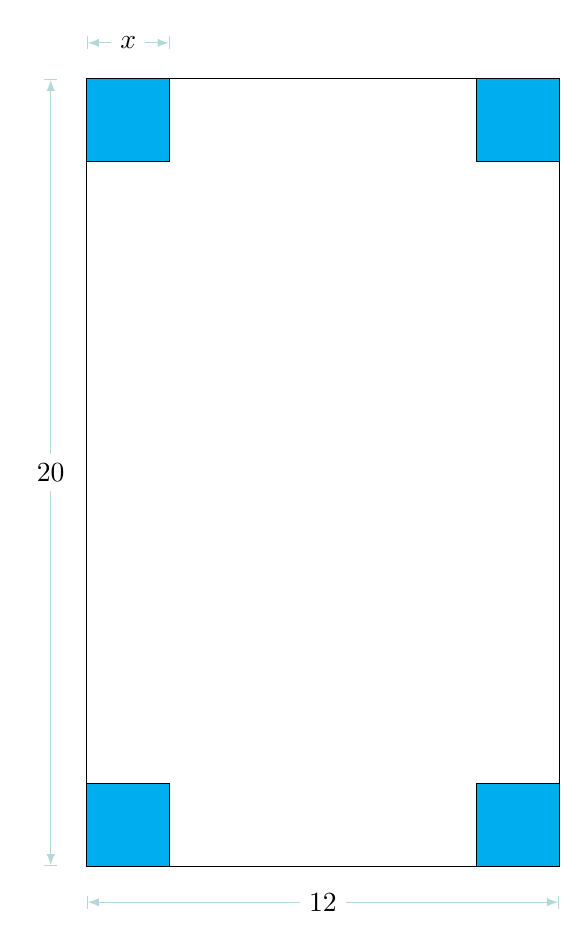
\begin{tikzpicture}[x=.5cm,y=0.5cm,>=latex]
\def\RWd{12}
\def\RHt{20}
\def\CutSide{30pt}
\draw
  (0,0) rectangle (\RWd,\RHt);
\path[draw,fill=cyan]
  (0,0) rectangle ++(\CutSide,\CutSide) 
  (\RWd,0) rectangle ++(-\CutSide,\CutSide) 
  (0,\RHt) rectangle ++(\CutSide,-\CutSide) 
  (\RWd,\RHt) rectangle ++(-\CutSide,-\CutSide);
\begin{scope}[|<->|,help lines,text=black]
\draw
  ([yshift=-13pt]0,0) -- node[fill=white] {$12$} ([yshift=-13pt]\RWd,0);   
\draw
  ([xshift=-13pt]0,0) -- node[fill=white] {$20$} ([xshift=-13pt]0,\RHt);   
\draw
  ([yshift=13pt]0,\RHt) -- node[fill=white] {$x$} ++(\CutSide,0);   
\end{scope}
\end{tikzpicture}

Para um determinado lado, devemos ter $x$ positivo 
\begin{eqnarray*}
		12-2x &>& 0\\
		-2x &>& -12\\
		2x &<& 12\\
		x &<& 6\\
\end{eqnarray*}
ou
\begin{eqnarray*}
		20-2x &>& 0\\
		-2x &>& -20\\
		2x &<& 20\\
		x &<& 10\\
\end{eqnarray*}

Em qualquer caso, $x$ deve ser positivo e menor que $6$, devemos ter: $x\in (0,6)$.

}

\qst{
{\bf Questão 47} 

O resto da divisão do polinômio $p(x)$ por $x-1$ é igual a $5$. Dividindo o mesmo polinômio
 por $x+1$, obtém-se o mesmo resto: $5$. Dividindo o polinômio $p(x)$ por $(x-1)\cdot (x+1)$, o resto obtido é:
\begin{multicols}{2}
\begin{enumerate}
		\item ( ) $0$.
		\item ( ) $5$.
		\item ( ) $25$.
		\item ( ) $125$.
		\end{enumerate}
\end{multicols}

}
\SOL{
Temos que 
\begin{eqnarray*}
		\begin{cases}
		p(x)=(x-1)q_1(x)+5\\
		p(x)=(x+1)q_2(x)+5
		\end{cases}
\end{eqnarray*}
Usando o Teorema do Resto:
\begin{eqnarray*}
		p(1)=5\\
		p(-1)=5\\
\end{eqnarray*}

Queremos determinar $R(x)$ na equação:
\begin{eqnarray*}
		p(x)=(x-1)(x+1)q(x)+R(x)
\end{eqnarray*}
Como $(x-1)(x+1)$ tem grau $2$, logo o resto $R(x)$ tem no máximo grau $1$ ,ou sejam $R(x)=ax+b$, reescrevendo:
\begin{eqnarray*}
		p(x)=(x-1)(x+1)q(x)+ax+b
\end{eqnarray*}
Aplicando os valores $p(1)$ e $p(-1)$:
\begin{eqnarray*}
		\begin{cases}
		p(1)=(1-1)(1+1)q(1)+a\cdot 1+b=a+b=5\\
		p(-1)=(-1-1)(-1+1)q(-1)+a\cdot (-1)+b=-a+b=5
		\end{cases}
\end{eqnarray*}
\begin{eqnarray*}
		\begin{cases}
		a+b=5\\
		-a+b=5
		\end{cases}
\end{eqnarray*}

Resolvendo o sistema, encontramos: $a=0$ e $b=5$. Portando, $R(x)=5$.

}
\todo{O teorema do Resto de Polinômios {\sc Afirma} que divisão de um polinômio $p(x)$ pelo binômio $ax+b$ tem como resto $p(\frac{-b}{a}$)}




%-----------------------------------------------------------
\listoftodos[Notes]
%-----------------------------------------------------------

\printbibliography
%-----------------------------------------------------------
\end{document}
